Para el desarrollo de esta práctica se utilizó el lenguaje de programación Python en su versión 3.10, con el que se diseñó un script para cumplir los objetivos de la práctica.


\subsection{Conjunto de datos utilizado}
El conjunto de datos utilizado en el desarrollo de esta práctica consta de información relacionada a la disponibilidad y precio de acciones NASDAQ. Dicho conjunto de datos consta de 5 atributos y 1 variable objetivo, sumando un total de 126 instancias sin presencia de datos faltantes.

Los atributos y la variable objetivo se puede categorizar de la siguiente forma:

\begin{itemize}
	\item Ordinales
		\begin{itemize}
			\item Date: Fecha del día correspondiente a la instancia.
		\end{itemize}
	\item Continuos
		\begin{itemize}
			\item Close/Last (variable objetivo): Precio al final del día.
			\item Volume: Cantidad de acciones disponibles.
			\item Open: Precio al iniciar el día.
			\item High: Precio más alto alcanzado durante el día.
			\item Low: Precio más bajo alcanzado durante el día.
		\end{itemize}
\end{itemize}


\subsection{Métricas para evaluación}
Tratándose del diseño de modelos de regresión que permitan predecir el valor futuro de las acciones NASDAQ, se optó por realizar una función que genera métricas para datos continuos de las predicciones realizadas por los algoritmos. Dicha función arroja las métricas mostradas a continuación:

\begin{itemize}
	\item Error cuadrático medio (MSE).
	\item Raíz del error cuadrático medio (RMSE).
	\item Error absoluto medio (MAE).
	\item Error cuadrático relativo (RSE).
	\item Coeficiente de correlación de Pearson (PCC).
	\item Coeficiente de determinación ($R^2$).
\end{itemize}


\subsection{Pre-procesamiento de datos}
\subsubsection{Limpieza de datos}
El conjunto de datos contenía observaciones en formato de texto, por ejemplo, para las observaciones del atributo \emph{Date} podíamos encontrar valores \emph{12/02/2022}, y para el caso de los atributos relacionados a precio podíamos encontrar valores como \emph{\$105.54}.

Para lidiar con los valores establecidos como texto de forma nativa, se diseñaron funciones que permiten convertir el atributo \emph{Date} a un formato de fecha nativo de Python, mientras que los atributos relacionados a precio se transformaron a valores tipo \emph{float}. Adicionalmente, se realizó un cambio en el orden de los datos, debido a que en un principio se encontraban de forma descendente (la fecha más reciente en la primer instancia).

Las Tablas \ref{Tab: InitialData} y \ref{Tab: ProcessedData} presentan una muestra de los datos originales del conjunto de datos (Tabla \ref{Tab: InitialData}) y el resultado del proceso de limpieza de datos (Tabla \ref{Tab: ProcessedData}).

\begin{table}[hp]
\centering
\caption{Datos originales}
\begin{tabular}{@{}llllll@{}}
\toprule
Date       & Close/Last & Volume   & Open     & High     & Low      \\ \midrule
12/02/2022 & \$105.05   & 7916878  & \$102.02 & \$105.54 & \$101.82 \\
12/01/2022 & \$103.37   & 7452313  & \$102.33 & \$103.56 & \$101.95 \\
11/30/2022 & \$102.2    & 15000770 & \$99.05  & \$102.56 & \$98.52  \\
11/29/2022 & \$98.66    & 4423921  & \$98.96  & \$99.33  & \$98.2   \\
11/28/2022 & \$98.66    & 5257862  & \$98.99  & \$100.16 & \$98.56  \\ \bottomrule
\end{tabular}
\label{Tab: InitialData}
\end{table}

\begin{table}[hp]
\centering
\caption{Datos transformados}
\begin{tabular}{@{}llllll@{}}
\toprule
Date       & Close/Last & Volume   & Open  & High    & Low   \\ \midrule
2022-06-06 & 78.98      & 7239429  & 79.70 & 81.2999 & 78.53 \\
2022-06-07 & 79.47      & 5517101  & 78.57 & 79.7500 & 78.26 \\
2022-06-08 & 78.47      & 5178253  & 78.90 & 79.7698 & 78.26 \\
2022-06-09 & 78.91      & 13248100 & 77.97 & 80.2700 & 77.73 \\
2022-06-10 & 75.67      & 8695476  & 77.02 & 77.7900 & 75.66 \\ \bottomrule
\end{tabular}
\label{Tab: ProcessedData}
\end{table}


\subsubsection{Normalización de datos}
Todos los atributos de tipo continuo se sometieron a un proceso de normalización, donde se utilizaron 2 métodos de normalización para datos continuos, normalización logaritmica (para el atributo \emph{Volume}) y normalización z-score para el resto de los atributos continuos (excluyendo la variable objetivo).

La elección del método de normalización para cada uno de los atributos se realizó mediante un análisis de la distribución de los datos de cada uno de los atributos, donde se llegó a determinar que los atributos relacionados con precios mostraban una tendencia a una distribución normal, mientras que el atributo \emph{Volume} mostraba una distribución sesgada positiva con valores en sus observaciones de la magnitud de millones.

Las Figuras \ref{Fig: open_dist} y \ref{Fig: volume_dist} muestran un ejemplo del proceso de normalización de los atributos continuos. Donde de lado izquierdo se puede observar las gráficas de distribución previas y posterior al proceso de normalización, mientras que del lado derecho se muestran los diagramas de caja correspondientes a los instantes antes mencionados.

\begin{figure}[hb]
	\centering
	\begin{subfigure}{\textwidth}
         \centering
         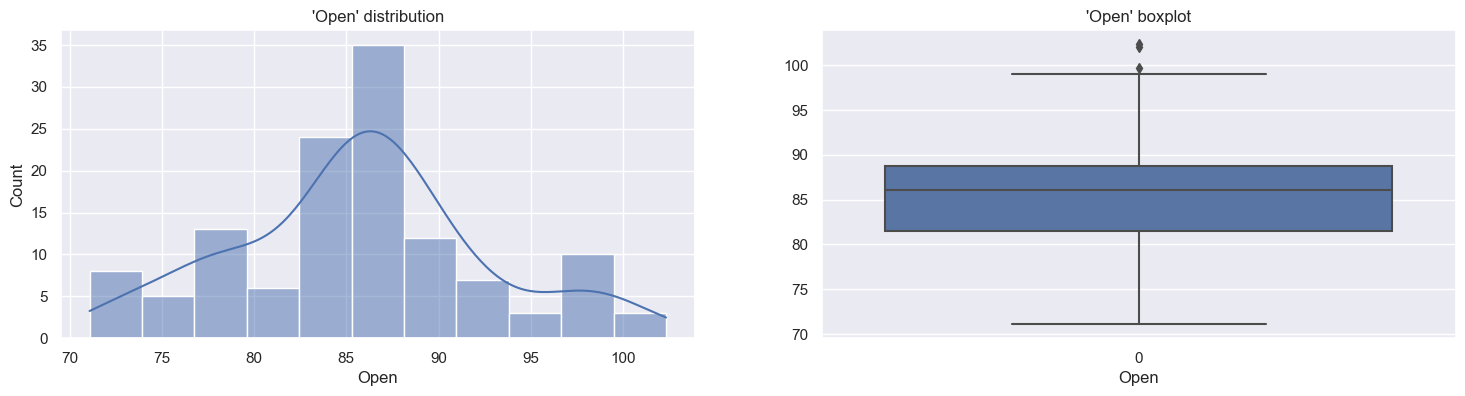
\includegraphics[width=\textwidth]{distribution_open}
         \caption{Distribución previa a normalizar.}
         \label{Fig: open_org}
	\end{subfigure}
	\vfill
	\begin{subfigure}{\textwidth}
         \centering
         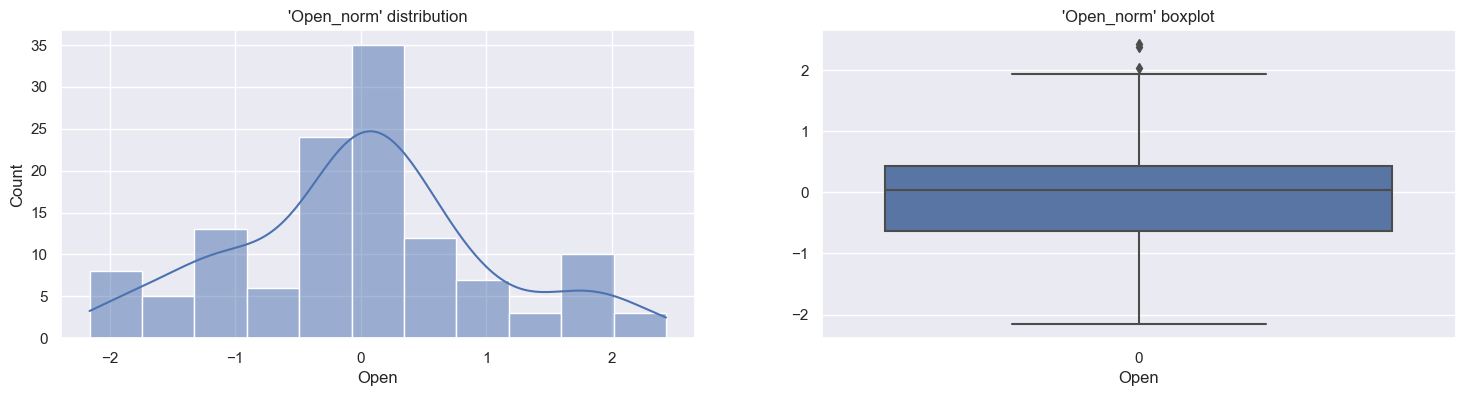
\includegraphics[width=\textwidth]{distribution_open_norm}
         \caption{Distribución posterior a normalizar.}
         \label{Fig: open_norm}
	\end{subfigure}
	\caption{Distribución de los datos del atributo \emph{Open}.}
	\label{Fig: open_dist}
\end{figure}

\begin{figure}[t]
	\centering
	\begin{subfigure}{\textwidth}
         \centering
         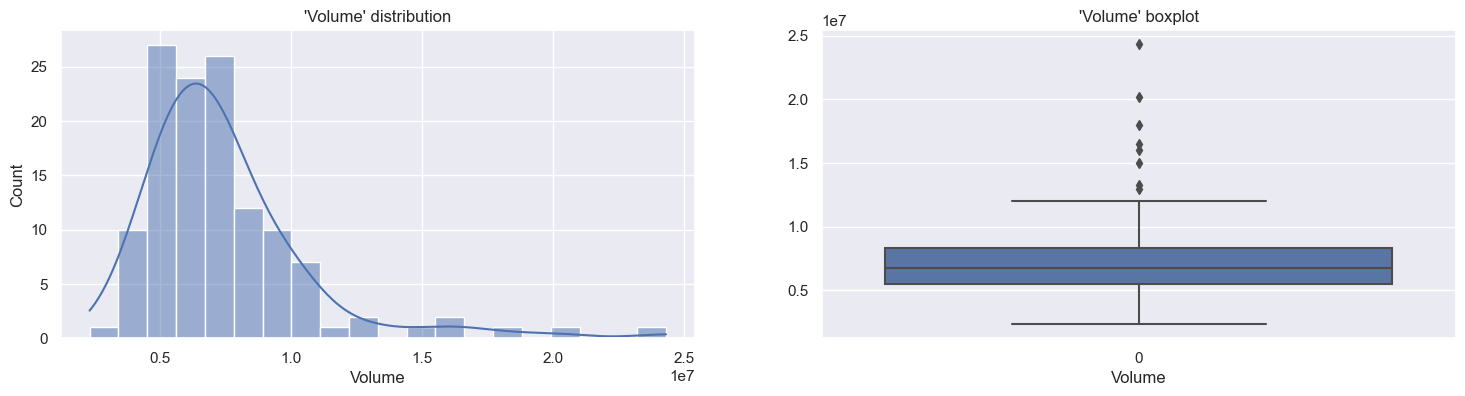
\includegraphics[width=\textwidth]{distribution_volume}
         \caption{Distribución previa a normalizar.}
         \label{Fig: volume_org}
	\end{subfigure}
	\vfill
	\begin{subfigure}{\textwidth}
         \centering
         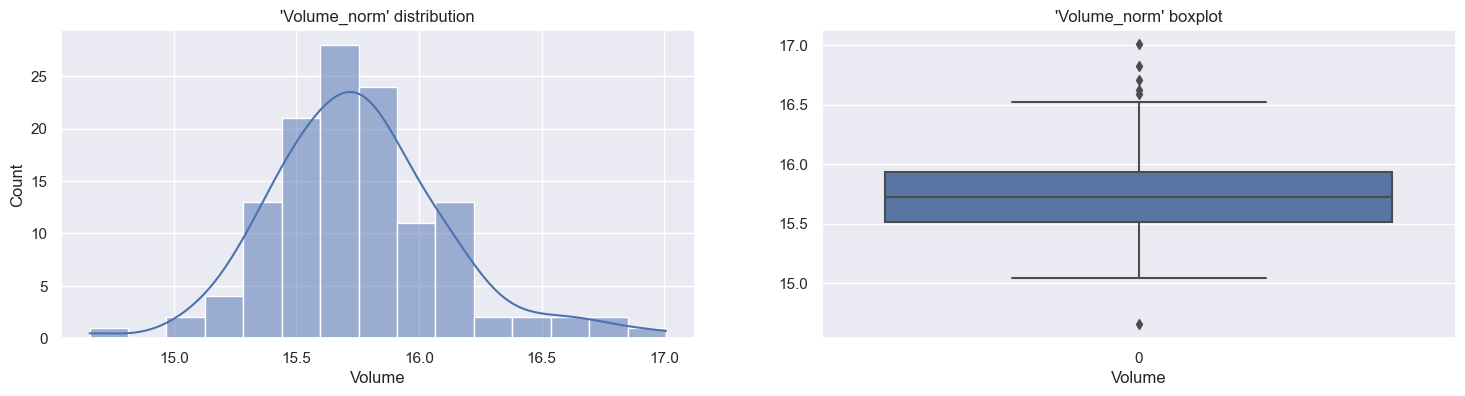
\includegraphics[width=\textwidth]{distribution_volume_norm}
         \caption{Distribución posterior a normalizar.}
         \label{Fig: volume_norm}
	\end{subfigure}
	\caption{Distribución de los datos del atributo \emph{Volume}.}
	\label{Fig: volume_dist}
\end{figure}



\subsubsection{Extracción de características}
Previo al desarrollo de los algoritmos de regresión se realizó un proceso de extracción de características, esto con el objetivo de seleccionar los atributos de mayor relación con la variable objetivo.

Junto con este proceso se realizó la segmentación del atributo \emph{Date} en dos atributos: \emph{Month} y \emph{Day}, esto con el objetivo de buscar relaciones cíclicas con la variable objetivo.

Mediante la obtención de un mapa de correlación (Figura \ref{Fig: heatmap}) se determinó que los atributos de mayor relación con la variable objetivo son: \emph{Open}, \emph{High}, \emph{Low} y \emph{Month}.

\begin{figure}[ht]
	\centering
	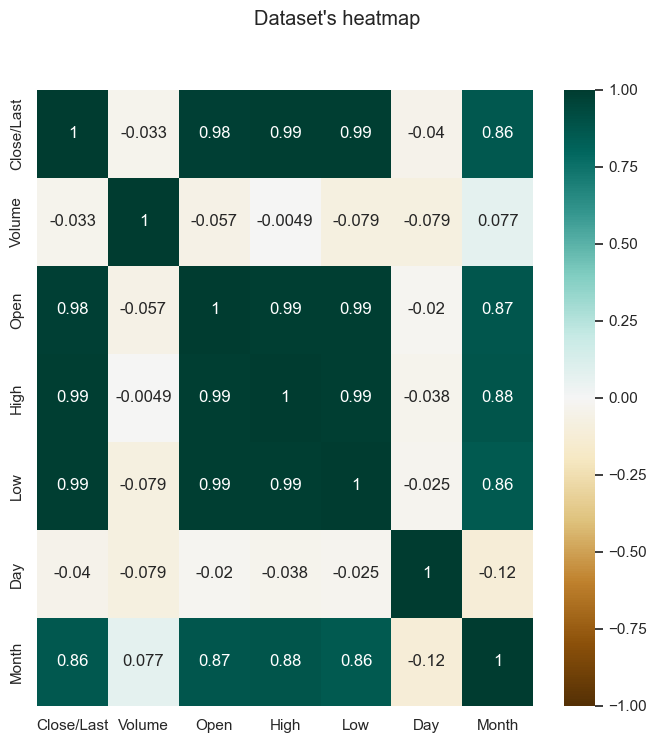
\includegraphics[width=0.6\textwidth]{dataset_heatmap}
	\caption{Mapa de correlación del conjunto de datos.}
	\label{Fig: heatmap}
\end{figure}

Una vez identificados los atributos de mayor relación con la variable objetivo, se procedió a segmentar el conjunto de datos en una proporción 80:20, tomando como conjunto de entrenamiento a las primeras 100 instancias del conjunto de datos, y las restantes 26 se designaron como conjunto de prueba. La Figura \ref{Fig: over_time} muestra la segmentación de estos datos en la variable objetivo.

\begin{figure}[hb]
	\centering
	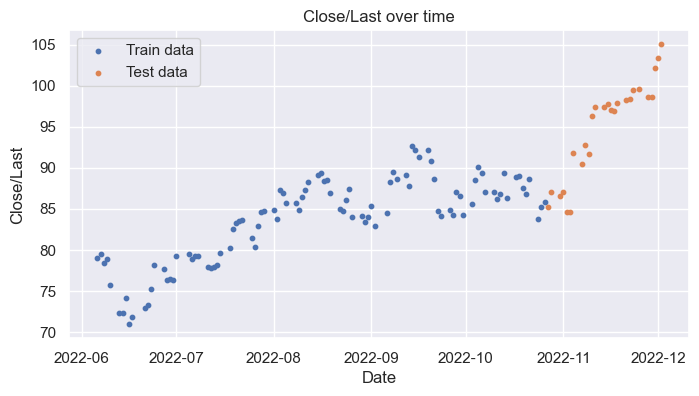
\includegraphics[width=0.7\textwidth]{closelast_time}
	\caption{Conjuntos de entrenamiento y prueba vistos respecto al tiempo.}
	\label{Fig: over_time}
\end{figure}


\FloatBarrier
\subsection{Algoritmos de regresión}
Enfocándose en uno de los objetivos principales de este trabajo, se implementaron 4 algoritmos de regresión, los cuales fueron:

\begin{itemize}
	\item Regresión lineal simple: Se selecciona debido a que tenemos atributos con alto nivel de correlación. Se seleccionará solamente uno para esta regresión.
	\item Regresión polinomial. Existe la posibilidad de que la relación entre la variable objetivo y los atributos de alta correlación no sea lineal. Se selecionará un atributo y se modelará como polinomio.
	\item Regresión lineal múltiple. Retomando el hecho de tener varios atributos con alta correlación, es muy probable que el utilizar todos esos atributos al mismo tiempo favorezca el desempeño.
	\item Regresión Ridge. Nos permite ajustar el modelo gracias al sistema de penalización, por lo que en casos como el nuestro (varios atributos con alta correlación) será benéfico para reducir los efectos de alta dimensionalidad.
\end{itemize}

Dichos algoritmos fueron evaluados con la metodología presentada en secciones anteriores.
